\documentclass{iopart}
\usepackage{iopams}

% Hack to be able to use amsmath
\expandafter\let\csname equation*\endcsname\relax
\expandafter\let\csname endequation*\endcsname\relax
\usepackage{amsmath}
% Note to the editor: It is a very unfortunate package incompatibility. Please fix this!

\usepackage{graphicx}
\usepackage{xcolor}
\usepackage{amssymb}
\usepackage{tikz}
\usepackage{adjustbox}
%\usepackage{natbib}

\usetikzlibrary{shapes,arrows,positioning}

\tikzstyle{block} = [draw, rectangle, fill=yellow!20,
    minimum height=2em, minimum width=3em, inner sep=0.5em]
\tikzstyle{sum} = [draw, circle, inner sep=0pt, minimum size=0.6em]
\tikzstyle{junction} = [draw, circle, fill, inner sep=0pt, minimum size=1mm]
% Uncomment the following to leave junctions "plain" (no small filled in circle):
\tikzstyle{coord} = [coordinate]
\tikzstyle{connector} = [->,thick]
\tikzstyle{tag} = [node distance=1mm]

\newcommand{\remark}[1]{\textcolor{blue}{[#1]}}

\newcommand{\gguide}{{\it Preparing graphics for IOP journals}}
\begin{document}

\title[Modeling and control of plasma rotation using NTV and NBI]{Modeling and control of plasma rotation for NSTX using Neoclassical Toroidal Viscosity and Neutral Beam Injection}

\author{I. R. Goumiri$^1$, C. W. Rowley$^1$, S. A. Sabbagh$^2$, D. A. Gates$^3$, S. P. Gerhardt$^3$, M. D. Boyer$^3$, R. Andre$^3$  E. Kolemen$^3$, K. Taira$^4$ }

\address{$^1$ Department of Mechanical and Aerospace Engineering, Princeton University, Princeton, NJ 08544, USA}
\address{$^2$ Department of Applied Physics and Applied Mathematics, Columbia University, New York, NY 10027, USA}
\address{$^3$ Princeton Plasma Physics Laboratory, Princeton, NJ 08544, USA}
\address{$^4$ Florida Center for Advanced Aero-Propulsion, Florida State University, Tallahassee, Florida 32310, USA}

\ead{igoumiri@princeton.edu}
\vspace{10pt}
\begin{indented}
\item[]June 2015
\end{indented}

\begin{abstract}
A model-based feedback system is presented to control plasma rotation in a
magnetically confined toroidal fusion device, to maintain plasma stability for
long-pulse operation.
%
This research uses experimental measurements from the National Spherical Torus
Experiment (NSTX) and is aimed at controlling plasma rotation using two
different types of actuation: momentum
from injected neutral beams and neoclassical toroidal viscosity generated by
three-dimensional applied magnetic fields.
%
Based on the data-driven model obtained, a feedback controller is designed, and
predictive simulations using the TRANSP plasma transport code show that the
controller is able to attain desired plasma rotation profiles given practical
constraints on the actuators and the available measurements of rotation.
\end{abstract}

\ioptwocol

%\maketitle

\section{Introduction}

Spherical tokamaks such as the National Spherical Torus Experiment (NSTX
\cite{Ono00}) are toroidal magnetic fusion devices that have been proven
experimentally to realize theoretical expectations of efficient and compact
advanced tokamak operation, producing high plasma pressures in relation to the
pressure of the magnetic field used to create the plasma equilibrium. In certain
circumstances, these high pressures can cause rapidly growing
magnetohydrodynamic (MHD) plasma instabilities that can lead to undesirable
effects such as reducing the plasma pressure, or even terminating the plasma (disruption).
%
Many of these instabilities are sensitive to the shear, so the rotation profile
plays a key role in regulating these instabilities.
%
The goal of the present study is to describe a model-based approach to
controlling the rotation profile in spherical tokamaks, and to apply the
approach to a predictive model based on experimental data from NSTX.

The effect of the rotation profile on MHD instabilities has been well studied in
recent years.  For instance, greater stability of tearing modes has been associated with
increased shear \cite{Gerhardt09, Park13}, while
rotation profile shapes that lead to stronger kinetic resonances lead to
stabilization of kink/ballooning modes and resistive wall modes \cite{Sabbagh10,
  Berkery10}. Furthermore, rotational shear can affect plasma turbulence and
consequently can have an impact on transport processes and the energy
confinement performance of tokamak plasmas. In present-day pulsed tokamaks,
plasma rotation can evolve, through normal heat and momentum transport
processes, toward profiles for which certain MHD modes are unstable.
%
Even if these profiles evolve by chance to a steady-state profile that is
stable, transient processes including Edge-Localized Modes (ELMs), internal transport
barriers, and different heating mechanisms can alter plasma profiles further and make
them less stable, or unstable \cite{Sabbagh13}.
%
In large fusion-power-producing tokamak operation (including ITER
\cite{Hender07}), disruptions caused by macroscopic instabilities can generate
electromagnetic forces and heat loads large enough to damage device components,
so it is particularly important to avoid such disruptions, for instance through
control of the rotation profile.

There is an abundant literature on plasma control such as kinetic profile control (density and temperature) \cite{Schuster02, Boyer11}, burn control \cite{Schuster01, Schuster02-2, Schuster02-3, Vitela98, Boyer12}, toroidal current profile control \cite{Boyer133, Boyer144, Barton12, Ou09, Ebrahimi04}, direct control of tearing modes \cite{Welander13, Volpe09} and resistive wall modes \cite{Sabbagh06,Sabbagh13}. Rotation control in tokamaks has been demonstrated using momentum input from injected neutral beams (NBI) as an actuator \cite{Scoville07}.  A new and unique aspect of the present work is the use of non-axisymmetric (three-dimensional) magnetic fields as another actuator in closed-loop feedback control to supplement the neutral beam actuator. Rotation alteration by non-resonant, three-dimensional magnetic fields allows more precise, continuous control of the plasma rotation alteration than NBI, as the momentum delivered by the latter occurs in significantly large, discrete increments.

The physical process creating the force on the plasma rotation generated by the applied three-dimensional field, termed neoclassical toroidal viscosity (NTV) \cite{Shaing88, Shaing10, Shaing15}, has been used successfully to affect plasma rotation in a pre-programmed manner on NSTX over a wide range of plasma operation, with quantitative agreement of the experimentally generated torque to theory \cite{Zhu06}. NTV is caused by non-ambipolar diffusion of plasma ions and electrons caused by the magnetic field components that break the usual toroidal symmetry of tokamak confinement field. As NTV depends on several important plasma parameters including temperature, and the plasma rotation itself, its use in closed-loop feedback leads to weak nonlinearities which must be investigated to ensure successful control. Details of such elements will be shown throughout this work. 

The present work defines a model-based algorithm for plasma rotation control
based on experimental data from NSTX \cite{Ono00}, that measures the rotational
(toroidal) momentum transport in the tokamak.  Data-driven modeling techniques
have been successfully used in the past to model plasma transport dynamics for
active control design in fusion reactors \cite{Moreau13, Boyer133, Boyer144,
  Barton12}. A novel contribution of this work is the development of a
one-dimensional partial differential equation model that is computationally
inexpensive, and may therefore implemented for real-time control.
%
The present simplified model of plasma momentum transport retains the most
important elements of the plasma momentum balance, including the effects of NBI
and NTV, and reproduces the general features of the plasma rotation evolution
measured in experiments.

Once the model is satisfactorily developed, a further step consists of applying
a spectral decomposition method, linearizing the equation about an equilibrium
and projecting onto a subspace spanned by Bessel functions, in order to obtain
an approximate linear model consisting of just 5 ordinary differential
equations.
%
The resulting reduced model is then used to design a controller using standard
techniques from optimal control.
%
The advantage of using a reduced-order model is that the resulting controller is
also low dimensional, so that it is computable in real time, as well as being
easier to tune and design.
 
The paper is organized as follows.  Section~\ref{MHW} describes the data-driven model
definition with details about the actuators used, model reduction process and
comparison to experimental data. Section~\ref{LRPC} describes the optimal
control method used to track a desired rotation profile, using both NTV and NBI
as actuators, and its implementation through numerical simulation. Section~\ref{sec:sim_results}
presents the results of the designed controller on a more complete rotation
model that can be found in TRANSP, a time dependent code developed at Princeton
Plasma Physics Laboratory for both prediction and analysis of tokamak
experimental data \cite{Goldston81, Budny94}. Conclusions and future work are
discussed in Section~\ref{sec:conclusions}.


 \section{A simplified model of  the toroidal momentum balance }
 \label{MHW}
 
\subsection{Model definition}
Consider the transport of toroidal angular plasma momentum in a tokamak with the assumption of axisymmetry.  To facilitate the analysis, an arbitrary flux surface average $\rho \in [0,1]$ is used, where $\rho = 0$ and $1$ denote the center and the boundary of the plasma, respectively.  

Using the work of Goldston \cite{Goldston86}  and Callen  \cite{Callen09}, the angular velocity of the plasma $\omega$ can be described dynamically by the flux surface average $\left<\cdot\right>$ of the toroidal momentum equation 
\begin{multline}
  \sum_i n_i m_i \left<R^2\right> \frac{\partial \omega}{\partial t}
  + \omega \left<R^2\right> \sum_i m_i \frac{\partial n_i}{\partial t} \\
  + \sum_i n_i m_i \omega \frac{\partial \left<R^2\right>}{\partial t} \\
  + \sum_i n_i m_i \left<R^2\right> \omega \left( \frac{\partial V}{\partial\rho}\right)^{-1} \frac{\partial}{\partial t} \frac{\partial V}{\partial \rho} \\
  = \left( \frac{\partial V}{\partial\rho}\right)^{-1}\frac{\partial}{\partial \rho} \left[\frac{\partial V}{\partial \rho}\sum_i n_i m_i \chi_\phi \left< R^2 (\nabla \rho)^2\right> \frac{\partial\omega}{\partial\rho}\right] \\
  - \left( \frac{\partial V}{\partial\rho}\right)^{-1}\frac{\partial}{\partial \rho} \left[\frac{\partial V}{\partial \rho}\sum_i n_i m_i \omega \left< R^2 (\nabla \rho)^2\right> \frac{v_\rho}{|\nabla\rho|}\right] \\
  - \sum_i n_i m_i \left< R^2\right> \omega \left( \frac{1}{\tau_{\phi cx}} + \frac{1}{\tau_{c\delta}}\right) + \sum_j T_j.
	\label{eq:full1}
\end{multline}
The left-hand side of the equation above represents the temporal change in the plasma toroidal angular momentum and the right-hand side terms denote respectively the one-dimensional fluid viscous term, pinch term, momentum loss due to charge exchange and field ripple, and the torque inputs (i.e., neutral beam injection and neoclassical toroidal viscosity). $R$ is a major radial coordinate, $\partial V/\partial\rho$ is the differential flux surface volume, $\chi_\phi$ is the perpendicular (to the equilibrium magnetic field) momentum diffusivity, $\tau_{\phi c x}$ and $\tau_{c\delta}$ are the time scales of the local momentum loss associated with charge-exchange and field ripple, $T_j$ represents the various torques acting on the system, $n_i$ is the particle density and $m_i$ is the particle mass for each particle species, but for simplicity, only the main plasma ion species (deuterium) are considered in the dynamics.

It is assumed that the plasma cross-sectional shape is well controlled by a
separate control loop; therefore $\left< R^2 \right>$, $\left< R^2
  (\nabla\rho)^2 \right>$, and $\partial V/\partial \rho$ are held fixed.
Curve-fits from time-averaged values of these functions (4th (Figures~\ref{fig:geofunc}(\emph{a}) and (\emph{c})), 5th (Figures~\ref{fig:geofunc}(\emph{b}) and (\emph{d})) order
polynomials or cubic spline (Figure~{\ref{fig:chiphi}}) interpolation depending on which one gives the smoothest fit) from TRANSP analysis of an experimental
plasma are used as approximations.
%
Representative data for a plasma discharge (133367) is shown in
Figures~\ref{fig:geofunc}(\emph{a}), \ref{fig:geofunc}(\emph{b}) and
\ref{fig:geofunc}(\emph{c}) respectively.  As it can be seen, the temporal
fluctuations of these variables are small. Hence taking the time-average values
or even the fixed values at an adequately chosen time ($t = 0.65 s$) is
considered to be a close approximation.
%
\begin{figure} 
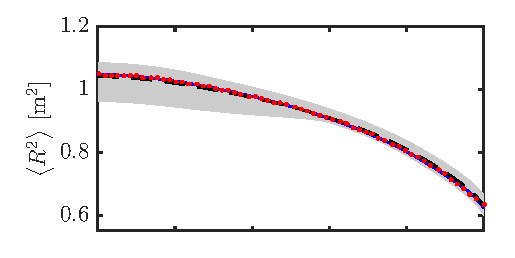
\includegraphics{imene_figs/fig1a} \hspace{-3em}\raisebox{7.7em}{(a)} \\
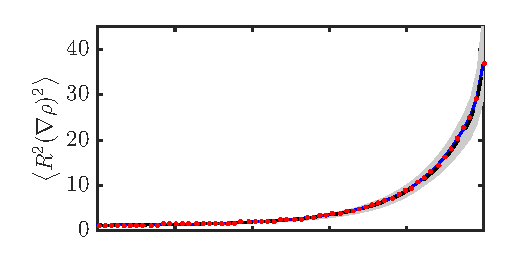
\includegraphics{imene_figs/fig1b} \hspace{-3em}\raisebox{7.7em}{(b)} \\
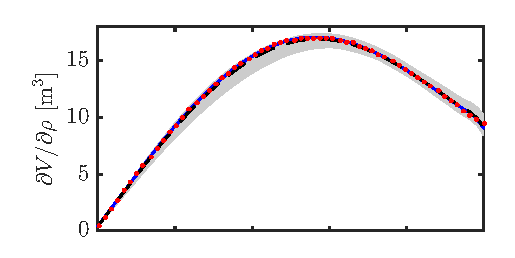
\includegraphics{imene_figs/fig1c} \hspace{-3em}\raisebox{7.7em}{(c)} \\[-.4em]
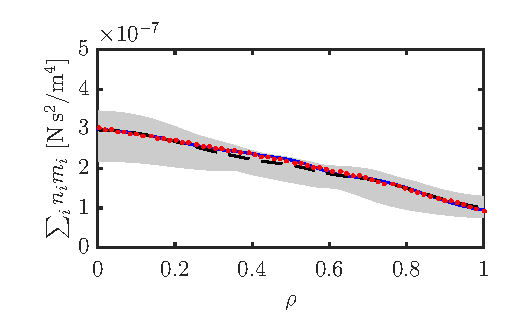
\includegraphics{imene_figs/fig1d} \hspace{-3em}\raisebox{9.7em}{(d)}
\caption{Functions describing the radial profiles of the geometrical properties: $\left< R^2 \right>$, $\left< R^2 (\nabla\rho)^2 \right>$, $\partial V/\partial \rho$ and  the mass density $ \sum_i n_i m_i $ from a TRANSP analysis of plasma discharge 133367.  The shaded region represents the value of the function spanned over time interval ($0.45$--$0.92$) seconds . The time-average values are shown by the black dashed line (--~--), the fixed time values and its curve-fit are shown by the solid blue lines (---) and the red dots (o) respectively.}
\label{fig:geofunc}
\end{figure}

It is also assumed for simplicity that the time variation of the mass density is
small.  This is a reasonable approximation, especially towards the edge ($\rho=1$), as seen in Figure~{\ref{fig:geofunc}}(\emph{d}).
This assumption may later be removed allowing $ \sum_i n_i m_i $  to vary in
time for more complex time-dependent systems, but for now, it allows the density
time derivative term in the left-hand side of equation~(\ref{eq:full1}) to be
neglected, resulting in a time-invariant system that is more amenable to control
design.
 
 Incorporating these observations into equation~(\ref{eq:full1}), we obtain a simplified diffusion equation
\begin{multline}
 n m \left<R^2\right>
 \frac{\partial \omega}{\partial t} \\
 = \left( \frac{\partial V}{\partial\rho}\right)^{-1}
   \frac{\partial}{\partial \rho} 
   \left[\frac{\partial V}{\partial \rho} n m \chi_\phi 
   \left< R^2 (\nabla \rho)^2\right> 
   \frac{\partial\omega}{\partial\rho}\right] \\
   \hfill + T_\text{NBI} + T_\text{ NTV},
		\label{model0}
\end{multline}
with boundary conditions
\begin{equation}
\left.\frac{\partial\omega}{\partial\rho}\right|_{\rho=0} = 0 
\quad \text{and} \quad 
\left.\omega\right|_{\rho=1} = 0.
\label{bc0}
\end{equation}
Here, $T_\text{NBI} $ and $T_\text{NTV}$ represent the torques
arising from neutral beam injection (NBI) and neoclassical toroidal viscosity
(NTV). Note that for this significant class of high confinement discharges, the
pinch term and  the momentum loss due to charge exchange are small and the
momentum loss due to  field ripple is not required, as NTV is explicitly
determined in this calculation. Details of the models for $T_\text{NBI}$
and~$T_\text{NTV}$ are shown in sections~\ref{NBIAM} and~\ref{TNTV}.  The
Dirichlet boundary condition at the plasma edge ($\rho=1$) is chosen to be
consistent with experimental observations.
  
A few observations can be made about this simplified model: first, equation  (\ref{model0}) is parabolic, ensuring the state operator to be negative definite (all eigenvalues are negative);  hence the system is stable, which is a desirable feature from a control viewpoint. 
Second, this approach captures only the momentum balance for rotation control and does not model potential plasma instabilities.
  
A key parameter in the model is the diffusion coefficient $\chi_\phi$, which we
take to be constant in time in~(\ref{model0}).
There are no direct measurements of $\chi_\phi$ inside the tokamak, but TRANSP
is able to reconstruct a value for $\chi_\phi$ for an experiment where $\omega$
is measured.
%
Figure~{\ref{fig:chiphi}} shows the deduced $\chi_\phi$ from a particular run (plasma discharge number~133775). This run is identical to the plasma discharge number~133367 except that it does not have an applied non-axisymmetric field, and therefore $T_\text{NTV} = 0$. This feature is very important because each dissipation effect needs to be considered separately from each source in the model. The data driven model will use the $\chi_\phi$ of discharge (133775) as its momentum diffusivity coefficient reference.


\begin{figure}
\centering
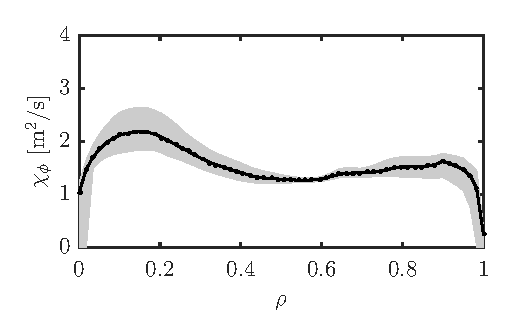
\includegraphics{imene_figs/fig2} % CHIPHI1n
\caption{The momentum diffusivity coefficient $ \chi_{\phi}$ is calculated through TRANSP analysis. The time-average values and their curve-fits are shown by the circles  and the solid lines respectively}
\label{fig:chiphi}
\end{figure}


The approach here is as follows: given a range of desired profiles that
the operator wishes the system to reach and stabilize,
take the simplified model~(\ref{model0}) that relies on different models of $ n  m$,
NTV and NBI torques from a representative class of plasma discharge ($\chi_\phi$ modeled from plasma discharge 133775),
linearize the model around an equilibrium whose basin of attraction contains the range of desired profiles
and use the linearized model to design a controller that will attempt to match any target shape within this range.

\subsection{Actuator models}

In order to control the toroidal momentum of the plasma in a spherical tokamak, we consider the use of two actuator mechanisms, namely, the neutral beam injection (NBI) and the neoclassical toroidal viscosity (NTV). The neutral beams are the main sources of momentum for the plasma and the NTV actuator is primarily used as a source of drag on the plasma. For NSTX, $T_\text{NBI}$ is strongest  in the plasma core, whereas $T_\text{ NTV}$ is strongest closer to the edge of the plasma. The momentum diffusivity $\chi_\phi$ allows transport of the momentum across these plasma regions on the momentum diffusion timescale of about $0.1\,s$ in NSTX H-mode plasmas.


\subsubsection{Neutral Beam Injection (NBI)}
 \label{NBIAM}

In NSTX, neutral beam injection is the main method to produce positive torque to increase plasma rotation, which is achieved  by injecting high-speed neutral atoms into the center of the plasma. 
Neutral atoms are able to cross the confining magnetic field of the tokamak without being deflected, and are ionized in the plasma via collisions with ions and electrons. The fast ions that are generated are also confined in the magnetic field and are able to exchange their energy to plasma ions and electrons. Typical injection acceleration voltages are in the range of 50\,keV to 130\,keV and for comparison, in NSTX, the peak plasma ion thermal temperature reaches up to $1.5$ keV.
Figure~{\ref{NBI_pics}} shows the planned neutral beam injection for the present
upgrade of NSTX. In the present study, we consider the three neutral beam
sources injected from the injector shown on the left of the figure.
Furthermore, for simplicity, we model the three sources as a single torque
input, as we describe below.

\begin{figure}
\begin{tabular}{cc}
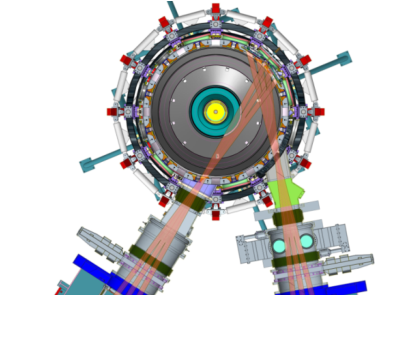
\includegraphics[width=\linewidth]{imene_figs/fig3a} \\
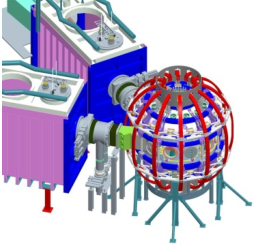
\includegraphics[width=\linewidth]{imene_figs/fig3b}
\end{tabular}
\caption{Illustration of the neutral beam injection (NBI) devices for NSTX-U with an inside view from the top of the tokamak (top) and outside view (bottom).}
\label{NBI_pics}
\end{figure}


A differential-equation model is introduced to relate the input power to the generated torque.  First, we approximate the NBI torque as a product of the spatial average of the torque, $\overline{T}_\text{NBI}(t) \equiv \text{avg}_\rho T_\text{NBI}(t,\rho)$, and a function, $F_\text{NBI}(\rho)$, that represents the spatial profile
\begin{equation}
   T_\text{NBI}(t,\rho) = \overline{T}_\text{NBI}(t) F_\text{NBI}(\rho),
\label{eq5}
\end{equation}
where the spatial profile of the torque is taken to be a Gaussian function (based on TRANSP analysis of NSTX discharge 133367) written as
\begin{equation}
F_\text{NBI}(\rho) = a_\text{NBI} \exp\left( - \frac{\rho^2}{2\sigma^2_\text{NBI}}\right).
\label{eq6}
\end{equation}
%
\begin{figure}
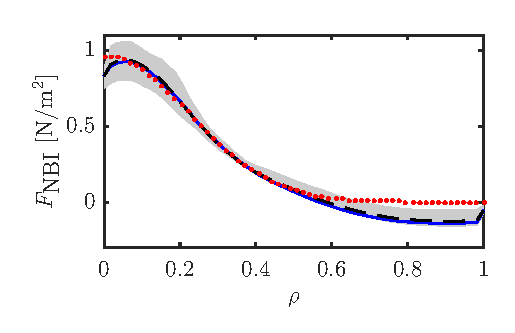
\includegraphics{imene_figs/fig4a} \hspace{-2.7em}\raisebox{12.2em}{(a)} \\[-1em] % Goum7
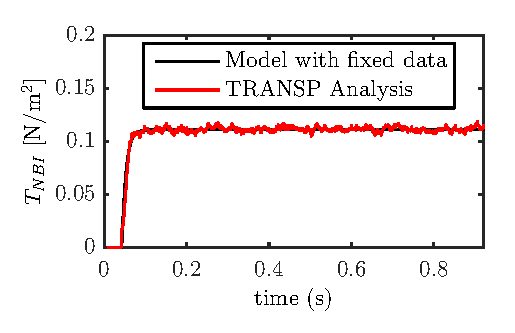
\includegraphics{imene_figs/fig4b} \hspace{-2.7em}\raisebox{4.2em}{(b)}          % Goum8
\caption{(a) Spatial profile for the neutral beam torque ($F_\text{NBI} $) for
  plasma discharge 133367.  The shaded region represents the values for times
  ranging from 0.45 to 0.92~seconds: time averaged values (--~--); values at the
  fixed time $t=0.6$s  (\textcolor{blue}{--~$\cdot$}); and
  the fit~\eqref{eq6} (\textcolor{red}{---}).
  %
  (b) Spatial average of the torque generated for the same plasma discharge
  ($ \overline{T}_\text{NBI}$), showing the TRANSP analysis
  (black) and the model~\eqref{eq:nbi_time} (red),
  %
  with
  $\tau_\text{NBI} = 0.01\,\text{s}$ and  $\kappa_\text{NBI} =
  2\times10^{-6} $.}
\label{fig:Fnbi}
\end{figure}
%
Figure~{\ref{fig:Fnbi}}(\emph{a}) shows the deduced profile $F_\text{NBI}$ of
the torque generated by the neutral beams, where the parameters
$a_\text{NBI}= 7.9090$
and~$\sigma_\text{NBI}= 0.2219$ were determined by a least-squares fit to the
time-averaged data.

In our model, the spatial average of the torque $\overline{T}_\text{NBI}(t)$ is
related to the power input, $P_\text{NBI}(t)$, by a first-order lag:
%
\begin{equation}
   \frac{\partial \overline{T}_\text{NBI}}{\partial t}
   + \frac{\overline{T}_\text{NBI}}{\tau_\text{NBI}}  = \kappa_\text{NBI} P_\text{NBI}(t),
   \label{eq:nbi_time}
\end{equation}
%
where $\tau_\text{NBI}$ is the approximate slowing down time of the fast neutral
beam particles to impart energy to the bulk plasma and $\kappa_\text{NBI}$ is a
scalar used to normalize the neutral beam power $P_\text{NBI}$.
%
Figure~\ref{fig:Fnbi}(\emph{b}) shows the solution of
equation~(\ref{eq:nbi_time}) with $P_\text{NBI}$ fixed to 6\,MW, compared with
the neutral beam torque predicted by TRANSP analysis, which uses a more
elaborate Monte Carlo model.
%\begin{figure}
%\centering
%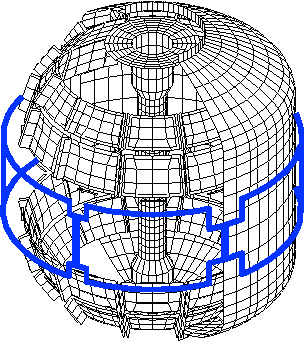
\includegraphics{imene_figs/fig5} % Goum9
%\caption{Comparison of the time evolution profile between the modeled NBI torque (from equations \ref{eq5}, \ref{eq6} and \ref{eq:nbi_time}) and the measured NBI torque from the TRANSP analysis.}
%\label{fig:Fullnbi}
%\end{figure}



\subsubsection{Neoclassical Toroidal Viscosity (NTV)}
 \label{TNTV}

Tokamaks usually have error fields or magnetohydrodynamic (MHD) activities present and these imperfections break the toroidal symmetry of the magnetic field and result in enhanced neoclassical toroidal plasma viscosity which then increases the rate of toroidal flow damping. The result will be a change of the edge rotation and shear. 

\begin{figure}
	\centering
   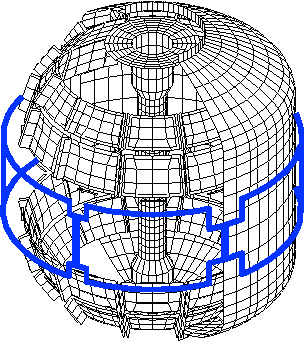
\includegraphics{imene_figs/fig5}
\caption{Model representation of the three-dimensional coils (highlighted in
  blue) used to create the magnetic field that produces NTV in the NSTX device.}
  \label{pic_NTV}
\end{figure}
For the current one-dimensional toroidal momentum model, we aim to model the momentum loss due to the neoclassical toroidal viscosity in the toroidal average sense and base our model on the work done in \cite{Zhu06} from which we can design the NTV torque as the bilinear product of the coil (Figure~\ref{pic_NTV}) current squared ($ I^2$) with the toroidal momentum $\omega$ as follows
\begin{equation}
   T_\text{NTV}  (t, \rho) =  - K \, G(\rho) \,  \langle R^2 \rangle \:  I^2(t) \,\omega (t, \rho),
    \label{eqn:ntv}
\end{equation}
where $K$ is a constant and $G$ is a Gaussian function.
\begin{figure}
	\centering
	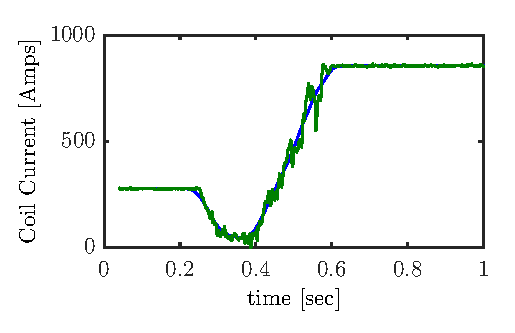
\includegraphics{imene_figs/fig6} \adjustbox{raise=10.2em, lap=-16em}{} % current
	\caption{ Coil current $I(t)$ for plasma discharges 133367:
          the green line represents the model from CHERS data and  blue lines represent the smoothed data.}
	\label{fig:current}
\end{figure}
The present model  will focus on the torque generated by the $n=3$ applied field ``configuration,'' in which the current reverses direction in each of the six neighboring coils. Other applied field configurations are possible (e.g., configurations with dominant $n = 2$ component) and have experimentally produced effective NTV as well \cite{Sabbagh10}.
 
The approach in our model is to approximate the general shape of $T_\text{NTV}/\omega$ by a time-invariant spatial profile and a time-evolution of a scalar current, similar to the way $T_{NBI}$ was treated. The resulting model has the form  
\begin{equation}
   \frac{T_\text{NTV}(t,\rho)}{\omega(t,\rho)} = - G_\text{NTV}  (\rho) \, I^2(t),
\end{equation}
where
\begin{equation}
G_\text{NTV}  (\rho) = K \,  \langle R^2 \rangle \:G(\rho),
\end{equation}
%
\begin{figure}
\centering
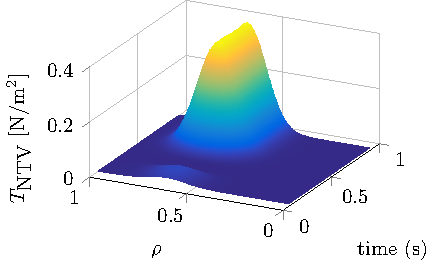
\includegraphics{imene_figs/fig7} % Goum10
\caption{3D representation of the NTV torque model~\eqref{eqn:ntv} where
  $\omega$ is taken from experimental measurements of ``fixed'' plasma discharge
  133367, and $I^2$ is as shown in Figure~\ref{fig:current}.}
\label{TNTV3D}
\end{figure}
%
and $G(\rho)$ is a Gaussian function centered towards the edge ($\mu =0.7, \sigma =0.1$).
%
Figure~{\ref{fig:current}}(\emph{a}) shows the current that flows into the coils
for the plasma discharge 133367. We notice that the current is kept constant
after $0.6$s. It should be noted that for control design, the actuator input
will be~$I^2(t)$.
%
Using the experimental rotation profile, the modeled NTV torque is shown in Figure~\ref{TNTV3D}.

\subsection{Testing and comparing the model}
\label{sec:test-comp-model}
In order to numerically simulate the partial differential equation~\eqref{model0}, we use a spectral method, projecting onto suitably chosen basis functions, to obtain a system of ordinary differential equations.  In particular, we write
\begin{equation}
\omega(\rho,t)  = \sum_{n=1}^{N} a_n(t) \varphi_n(\rho),
\label{decomp}
\end{equation}
where the basis functions are given by
\begin{equation}
  \label{eq:1}
  \varphi_n(\rho) = J_0(k_n\rho),\qquad n=1,\ldots,N,
\end{equation}
where $J_0$ denotes the Bessel function of the first kind and $k_n$ denotes the $n$-th root of $J_0$.  With this choice of basis functions, the expansion~\eqref{decomp} automatically satisfies the boundary conditions~\eqref{bc0}, both at $\rho=0$ (since $J_0'(0)=0$) and at $\rho=1$ (since $J_0(k_n)=0$).  Furthermore, the basis functions satisfy the orthogonality relation
\begin{equation}
  \label{eq:2}
  \langle \varphi_n,\varphi_m\rangle = 0,\qquad \text{for $m\ne n$},
\end{equation}
where the inner product is defined by
\begin{equation*}
\langle f,g \rangle =   \int^1 _0 \rho \, f(\rho) \, g(\rho) \, d\rho.
\end{equation*}
Note that~\eqref{model0} is linear in~$\omega$, and can be written as
\begin{equation}
\label{eq:3}
\partial \omega/\partial t=L(\omega,T_\text{NBI},T_\text{NTV}),
\end{equation}
where $L$ is a differential operator linear in each argument.  Inserting the expansion~\eqref{decomp} into~\eqref{eq:3}, taking inner products with~$\varphi_m$, and using the orthogonality relation~\eqref{eq:2} then gives
\begin{equation*}
  \dot a_m = \sum_{n=1}^N \frac{\langle L(\varphi_n, T_\text{NBI}, T_\text{NTV}),
    \varphi_m\rangle}{\langle \varphi_m,\varphi_m\rangle},\qquad m=1,\ldots,N,
\end{equation*}
which is a set of $N$ coupled ordinary differential equations for the coefficients $a_m$.

The parameters in the model~\eqref{model0} are determined from TRANSP analysis of plasma discharge 133367, as described in Section~\ref{MHW}.  Figure~\ref{Goum12} shows the comparison of the model with the TRANSP analysis (prediction of plasma discharge 133367), showing the rotation at two values, $\rho=0.1346$ and $0.5498$.
%
Given two points of measurements of rotation (outputs), one near the core, the other one towards the edge of the tokamak (more details in the next section); the model and TRANSP are first run with only the NBI actuator on ($6$\,MW), then at $t=0.5$\,s, the NTV actuator is turned on for both models with the same value. 

\begin{figure}
\centering
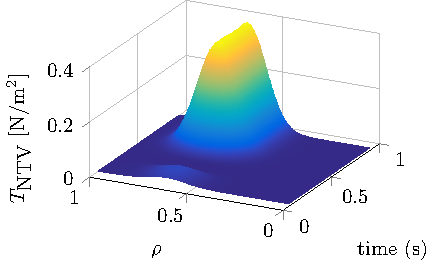
\includegraphics{imene_figs/fig8} % Goum12
\caption{Two rotation measurements with NBI and NTV actuators activated at $t=0$\,s and $t=0.5$\,s respectively, comparing TRANSP analysis with fixed background (black), with the model~\eqref{model0}, with $N=4$ Bessel functions (red).}
\label{Goum12}
\end{figure}

Figure~\ref{Goum12} shows these rotation measurements for the simplified model (red) compared against TRANSP analysis (solid black line) when the NBI and NTV actuators are activated at $t=0$\,s and $t=0.5$\,s respectively. The blue dashed line shows the steady values reached when only NBI is activated. It shows that the model is a good approximation of the TRANSP analysis model.


Figure~\ref{fig10} shows how the simplified model performs for a different plasma discharge ($133743$), at conditions different from those for which the model was calibrated.  The relative error between the reduced model and experimental data (which is the difference between the experimental and the model rotation divided by the mean of the spatial average of the experimental rotation data) is also shown in  the same figure.

For all the models, the initial condition is set to be the experimental rotational frequency at  time $t=0.4$\,s after the start up ($t=0$) and when the plasma reaches the H-mode.

An exact plasma model is not a major concern as feedback control can be performed to tolerate errors in the model. The key is to ensure the model does not deviate drastically from the actual profile in order to prevent control system instabilities from dominating plasma physics dynamics.

This simplified model (derived plasma discharge 133367) has been extensively validated against other plasma discharges in NSTX analysis (showing here 133743). The error remains acceptable starting with less than 25\% for the  experimental data 133743 where the original model was maintained the same, only the density and the input torques were updated. The error does not exceed 30\% for other experimental comparisons which is tolerable for plasma rotation control.

The overall behavior of the plasma is captured qualitatively very well using the simplified model of equation~\eqref{model0} with a fixed background. 

\begin{figure}
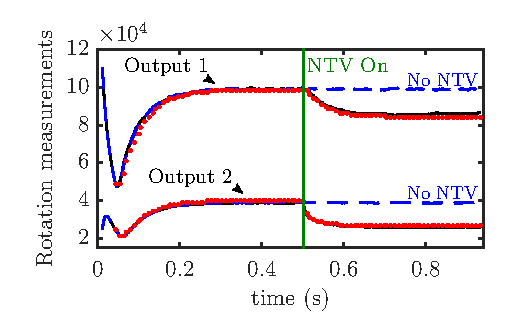
\includegraphics{imene_figs/fig9}
\caption{Comparison of the rotational frequency $\omega$ for plasma discharge 133743, comparing TRANSP analysis (left), with the simplified model~\eqref{model0}, projected onto $N=40$ Bessel modes, and $N=4$ Bessel modes.  Also shown is the relative error between TRANSP and the reduced model ($N=4$).}
\label{fig10}
\end{figure}


%\subsection{Reduced order model using Bessel functions}
%
%Among many model reduction techniques, such as singular perturbation or Hankel norm reduction methods, the projection-based method, which involves projection of a model onto a set of modes, is a widely used approach. These may be global eigenmodes of a linearized operator \cite{Akervik07}, modes determined by proper orthogonal decomposition (POD) of a set of data, or variants of POD modes \cite{Holmes12}. 
%
%It can be noticed from the mathematical structure of the momentum diffusion equation~(\ref{model0}), that the diffusion part looks like a Laplacian operator in cylindrical coordinates, thus the Bessel functions will be the natural choice for the basis. 
%
%Recall that the Bessel modes are constructed as different versions of the same Fourier-Bessel function of the first kind $J_{\alpha}$, where the argument to each version $n$ is differently scaled, according to
%\begin{equation}
%(J_{\alpha})_n (x) = J_{\alpha} \left(  \frac{ k_{\alpha,n}}{L} x \right),
%\label{defmod}
%\end{equation}
%where $ k_{\alpha,n}$ is a root, numbered $n$ associated with the Bessel Function $J_{\alpha}$.
%%
%\remark{The above is verbatim from the Wikipedia entry for Fourier-Bessel
%  series.  This is plagiarism, and is a major problem!  This needs to be
%  rewritten, and if there are other parts that are taken from other sources like
%  this, those need to be rewritten also.}
%%
%$L$ is a length constant assumed to equal unity as the spatial variable varies between 0 (at the core) and 1 (at the edge of the plasma). The variables $a_n$ are the assigned coefficients. The toroidal rotation $\omega$ can thus be written as 
%\begin{equation}
%\omega(\rho,t)  = \sum_{n=0}^{\infty} a_n(t) \, J_{\alpha} \left( { k_{\alpha,n}} \rho \right),
%\label{decomp}
%\end{equation}
% with
% \begin{equation}
%a_n(t) = \frac{\langle \omega(\rho,t), \left(J_{\alpha} \right)_n \rangle }{\langle  \left(J_{\alpha} \right)_n ,  \left(J_{\alpha} \right)_n   \rangle},
%\end{equation}
%and where the scalar product is defined as 
%\begin{equation}
%\langle f,g \rangle =   \int^1 _0 \rho \, f(\rho) \, g(\rho) \, d\rho.
%\end{equation}
%By matter of respecting the boundary conditions given in equation~(\ref{bc0}), we consider the particular case of $\alpha = 0$, this reduces equation~(\ref{decomp}) to
%\begin{equation}
%\omega(\rho,t)  = a_0(t) + \sum_{n=1}^{r} a_n(t) \, J_{0} \left(  k_{0,n} \rho \right),
%\end{equation}
%with
%\begin{equation}
%a_0 (t) = {2} \int^1 _0 \rho \, \omega(\rho,t) \, d\rho.
%\end{equation}
%and $r$ being the number of Bessel modes chosen to represent $\omega$.
%\remark{I don't think you should need the constant term.  In fact, if $a_0$ is nonzero, then the expansion~\eqref{decomp} will not satisfy the boundary condition at $\rho=1$ (since $J_0(k_{0,n})=0$).  Why is $a_0$ included?}
%
%This Bessel decomposition is now applied on the simplified model defined by equation~(\ref{model0}). Figure~\ref{bessel1} compares the three model simulations, one is taken from TRANSP analysis of the experimental measurement of the toroidal rotation (with varying background), the two other models are simulated in real space dimension and spectrally by projecting the original model on only 4 Bessel modes respectively in a fixed background. It can be noticed that only 4 Bessel modes are sufficient for capturing most features of the dynamics.
%
%\begin{figure}
%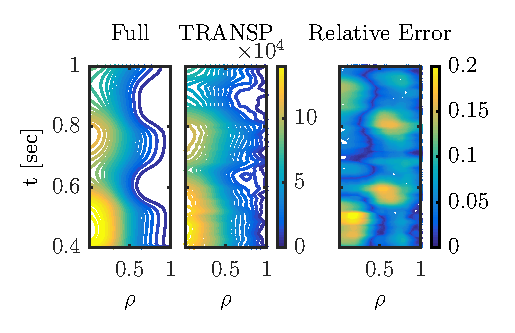
\includegraphics[width=\linewidth]{imene_figs/fig10} % bessel11n 
%\caption{comparison of spectral simulation of the toroidal rotation using 4 Bessel modes (right) with the full nonlinear simplified model using 60 points of discretization for plasma discharge 133367 (middle) in fixed background and the rotation from TRANSP analysis (left) in variable background.
%\remark{Not sure we need this figure.  What does this show that is not already in Figure 9?  I thought the point is that this model was calibrated on shot 133743 and run for shot 133367, then should make that point explicitly.}}
%\label{bessel1}
%\end{figure}
%
\section{Linear plasma rotation control}
 \label{LRPC}
 
 The purpose of this section is to demonstrate that standard model-based control techniques may be used to guide an experimental plasma rotation profile to track a desired reference. Some approaches on how controllers can be designed to achieve a desired profile with a reasonable response time are presented in the following sections.
 
 Recall that the two actuators available to the controller are the (NBI) beam power and the coil current producing NTV.
In this case, a state-space realization is derived and linear quadratic regulators are used to design a feedback controller that is optimal in minimizing a prescribed quadratic cost function.

\subsection{State space realization}
\label{SS}
In order to be able to use linear control tools, a state-space realization of equation~(\ref{model0})  shifted around a steady state has to be built.
Let $\bar{\omega}$ be the steady state reached for the given beam power $ \bar{P}$ and coil current $\bar{I}$. The linearization around this steady state profile can be written as
\begin{align}
\omega (t, \rho) &= \bar{\omega} (\rho) + \omega^{'}(t, \rho), \\
I (t) &= \bar{I} + I^{'}(t),\\
P_\text{NBI} (t) &= \bar{P} + P^{'}(t),
\end{align}
where $ \omega^{'}$ , $ I^{'}$ and $P^{'}$ are the respective perturbations to the equilibria $\bar{\omega}$, $\bar{I}$ and $\bar{P}$.
By plugging in these equations into equations~(\ref{model0}) and (\ref{eq:nbi_time}) and by linearizing equation~(\ref{eqn:ntv}) and simplifying, we obtain
\begin{multline}
	\frac{\partial}{\partial t}   \left[\! \begin{array}{c}  \omega^{'} \\ \overline{T}_\text{NBI} \end{array}\!\right]
		={ \left(\! \begin{array}{cc} a_{11}  & a_{12} \\ 0 & a_{22} \end{array} \! \right)} \left[\! \begin{array}{c} \omega^{'} \\ \overline{T}_\text{NBI}    \end{array}  \!\right] \\
		+ \left(\! \begin{array}{cc} b_{11}  & 0 \\ 0 & b_{22}    \end{array}  \!\right) \left[\! \begin{array}{c}  I^{'2}  \\ P^{'}\end{array}\!\right]
	\label{SSR}
\end{multline}
 where
 \begin{eqnarray}
 a_{11} =  \frac{1}{n m \left<R^2\right>} \Bigg[ \left( \frac{\partial V}{\partial\rho}\right)^{-1} \nonumber \\
   \hspace{-1em}\frac{\partial}{\partial \rho} 
   \left[\frac{\partial V}{\partial \rho}(n m)\chi_\phi 
   \left< R^2 (\nabla \rho)^2\right> 
   \frac{\partial}{\partial\rho}\right]-K G(\rho) \langle R^2 \rangle  I^2_0 \Bigg]  \nonumber \\
 a_{12} =  \frac{ F_\text{NBI}(\rho) }{n m \left<R^2\right>}\nonumber \\
 a_{22} = - \frac{1}{\tau_\text{NBI}}  \nonumber \\  
 b_{11} = - \frac{1}{n m \left<R^2\right>} K G(\rho) \langle R^2 \rangle  \omega_0 \nonumber \\
 b_{22} = \kappa_\text{NBI} \nonumber
 \end{eqnarray}
% 
This system of equations can be represented in the standard state-space form:
\begin{align}
	\dot{x} &= A x + B u, \label{eqn:state-space1} \\
	y &= C x, \label{eqn:state-space2} 
\end{align}
by using the spectral decomposition described in Section~\ref{sec:test-comp-model} and projecting the partial state $ \omega$ on the $r$ chosen Bessel functions, the perturbed state $x$ will then reduce to the $(r+1)$ Bessel coefficients of the projection $ \left[ a_{0}, a_{1}, ..., a_{r}  \ \ \overline{T}_\text{NBI}(t) \right]$.
%
%
$u \in \mathbb{R}^p$ is the perturbed input $\left( I^{'2}, \ \  P^{'} \right)$ and $y \in \mathbb{R}^q$ is the perturbed output (sensor measurements from their equilibrium values).
$A \in \mathbb{R}^{\, (r+1) \times (r+1)}$, $B \in \mathbb{R}^{\,(r+1) \times p}$, and $C \in \mathbb{R}^{\, q \times (r+1)}$ are respectively called the dynamics, control and sensor matrices.
Here, there are two actuators ($p=2$), one power input for the neutral beams and another one for the coil current producing the NTV.
The outputs $y$ correspond to the sensor measurements of the plasma toroidal rotation. Here, two measurements are taken, one near the core and one towards the edge of the plasma ($q=2$).
%
\subsection{Non-zero target state}
Once the state-space realization is obtained, the goal is to force the shape of the plasma rotation profile to reach a target state $x_d$ such that the sensor output $y$ matches a reference signal~$y_d$. In the final implementation, all one should have to prescribe is $y_d$ (e.g., plasma rotational frequency values at certain locations). The target state $x_d$ and the corresponding input $u_d$ are found by solving equations~(\ref{eqn:state-space1}) and (\ref{eqn:state-space2}) at steady state
\begin{equation}
\left[\! \begin{array}{c}  x_{d} \\ u_{d}\end{array}\!\right]
  ={ \left(\! \begin{array}{cc} A  & B \\ C & 0 \end{array} \! \right)}^{-1} \left[\! \begin{array}{c} 0 \\ I    \end{array}  \!\right] y_{d} = \left[\! \begin{array}{c} F_x \\ F_u    \end{array}  \!\right] y_{d}.
\label{steadystate}
\end{equation}
%and $\left( \bar{x}, \bar{u}  \right)$ is the equilibrium point around which the system is linearized, $\bar{y}$ the corresponding measurement values of $\bar{x} = \left( \bar{a}_{0},\, \bar{a}_{1},\ldots,\, \bar{a}_{r},\,\bar{T} \right)$. 
%
 
\subsection{Control design} 
Once the target states $\left( x_{d} , u_{d} \right)$ are established, the controllers are designed based on the reduced model dynamics, then applied to the full-dimensional linearized model, and finally tested on the original nonlinear model to determine if the controller can suppress disturbances and reach the desired profile in the vicinity of the equilibrium.


\subsubsection{Full-state feedback control design} 

When the reduced-order model (in Bessel basis) is obtained, a feedback control law can be constructed as
\begin{equation}
   u = u_{d} - K(x - x_{d}) = - Kx + Fy_{d},
   \label{eqn:ctrllaw_ff}
\end{equation}
where $K$ is the feedback control gain to be determined from control design and $F = F_u + K F_x$ is the feedforward gain.  Therefore, the resulting closed-loop system can be written as
\begin{equation}
\begin{aligned}
      \dot{x} &= (A-BK) x + BF y_{d}, \\
      y &= C x.
\end{aligned}\label{eq:4}
\end{equation}
In order to design the controller from equation~(\ref{eqn:ctrllaw_ff}), we have to choose the gains $K$.
A  standard linear control technique (linear-quadratic regulators) is used in order to determine those gains while minimizing a quadratic cost function of the form:
\begin{equation}
 \mathcal{J} = \int_{t_0}^\infty \left( x^T Q x + u^T R u \right) dt,
 \label{bel}
\end{equation}
where $Q\ge 0$ and $R>0$ are symmetric matrices chosen by the control designer. $Q$ will be chosen to be equal to $q \, C^{T} C$ where $q$ is a constant and $R$ is a $2 \times 2$ diagonal matrix, which reduces equation~(\ref{bel}) to
\begin{equation}
   \mathcal{J} = \int_{t_0}^\infty \left( q \, y^T y + u^T R u \right) dt.
\end{equation}

 
The input $u$, from equation~(\ref{eqn:ctrllaw_ff}), that minimizes $\mathcal{J}$ is obtained by setting
\begin{equation}
   K  = - R^{-1} B^T P,
\end{equation}
where $P$ is a positive-definite, symmetric matrix that solves the algebraic Riccati equation: $P {A} + {A}^T P - P {B} R^{-1} B^T P + Q = 0$.  This equation is solved numerically using standard routines in MATLAB. For more details about the method, see standard references such as~\cite{SandP, AandM}.
It should be noted that the feedforward gain~$F$  depends on the matrices $A$, $B$, $C$ and $K$.

Figure~\ref{fig:rot11} defines our initial profile, the equilibrium profile used for the linearization and the targeted profile where the measurements are done.
In this paper we use $q=10^{4}$ and $R=I$ by inspection of the magnitude of our inputs and outputs.
\begin{figure}
	\centering
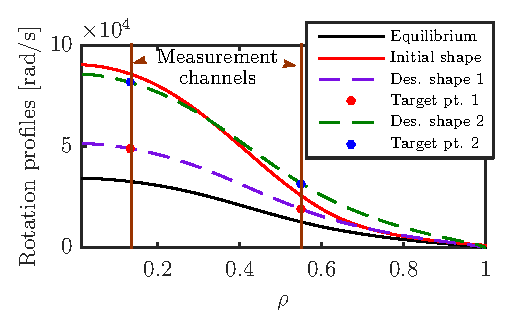
\includegraphics{imene_figs/fig11} % Goum133l
\caption{Rotation profiles: definition of the initial profile, equilibrium profile $w_0$ used for the linearization and the desired profiles to reach $w_d$. The two points of measurement $r$ are shown by the two dots.}
\label{fig:rot11}
\end{figure}




\subsubsection{Observer-based feedback control design} 

The feedback law~\eqref{eqn:ctrllaw_ff} we designed in the previous section requires knowledge of the full state~$x$.  However, in an actual experiment, we cannot measure the state directly; we measure only the outputs~$y$.  However, we may reconstruct an estimate of the state from the available sensor measurements using an {\em observer}.
A standard linear observer reconstructs a state estimate~$\hat x$, with dynamics given by
\begin{equation}
	\begin{split}
		\dot{\hat{x}} &=  A \hat{x} + B u + L (y - C \hat{x}) \\
			&= (A- L C) \hat{x} + B u + L y,
		\label{obs}
	\end{split}
\end{equation}
where the matrices $A,B$ and~$C$ are the same as those in the model~\eqref{eq:4}, and $L$ is a matrix of gains chosen such that the state estimate converges quickly relative to the system's dynamics.
Using our linear model, we design an optimal observer (Kalman filter) to find~$L$.
We introduce two zero-mean Gaussian white noise processes, $v$ the process disturbance and $w$ the sensor noise, with respective covariance matrices $V$ and~$W$, into equations \eqref{eqn:state-space1} and~\eqref{eqn:state-space2} to obtain
\begin{align}
	\dot{x} &= A x + B u + v, \label{eqn:state-space-noise1} \\
	y &= C x + w. \label{eqn:state-space-noise2} 
\end{align}
Then the expected variance of the error in the state estimate is obtained by setting
\begin{equation}
	L = P C^T W^{-1},
\end{equation}
where $P$ is a positive-definite, symmetric matrix that solves the algebraic Riccati equation: $A {P} + P {A}^T - P {C}^T W^{-1} C P + V = 0$.  This equation is solved numerically using standard routines in MATLAB. For more details about the method, see standard references such as~\cite{SandP, AandM}.
In this paper we use $V=10^{4}I$ and $W=10^{4}I$, corresponding to noise levels of approximately 1\% of the magnitude of our states and outputs.

The observer generates an estimate of the state from the physics model as represented by the state matrix, the inputs and outputs, and once combined to the feedback controller it forms a linear quadratic Gaussian compensator.

\subsubsection{Integrator, actuators saturation and anti-windup design} 

Because the primary goal is tracking the desired rotation profile, we want to minimize the steady state error between the output (measured) and the target profile. One way to handle such issue is to use integral action, introducing a new state variable~$z$ that is the integral of the error:
\begin{equation}
	\dot{z} = y - y_{d} = C x - y_{d}.
	\label{integral}
\end{equation}
The overall system can be then written as
\begin{multline}
\frac{\partial}{\partial t}   \left[\! \begin{array}{c}  x \\ z \end{array}\!\right]
  ={ \left(\! \begin{array}{cc} A  & 0 \\ C & 0 \end{array} \! \right)} \left[\! \begin{array}{c} x \\ z    \end{array}  \!\right] \\
  + \left(\! \begin{array}{c} B   \\ 0    \end{array}  \!\right) u -  \left(\! \begin{array}{c}  0 \\ I \end{array}\!\right) y_{d}
\label{int2}
\end{multline}
with a new feedback law designed as
\begin{equation}
u =   - \left(\! \begin{array}{cc}  K & K_I\end{array}\!\right) \left[\! \begin{array}{c}  x \\ z \end{array}\!\right] + F y_{d}
\end{equation}
where the gains $K$ and $K_I$ can be determined through the MATLAB command LQI.
A drawback of integral control is that if the actuator values are limited to some range $u\in[u_\text{min},u_\text{max}]$ (as they are in our case), then the integrator can accumulate error when the actuator is ``saturated,'' resulting in poor transient performance, a phenomenon known as ``integrator windup.''  We avoid these effects by using a standard anti-windup scheme (see, e.g., \cite{AandM, Lewis}), in which one feeds back the difference between the desired value of~$u$ and its actual (possibly saturated) value, as shown in the diagram in Figure~\ref{fig:model1}.  

Figure~\ref{fig:model1} shows the schematic of the overall controller, combining the feedback law~\eqref{eqn:ctrllaw_ff} with the observer~\eqref{obs}, the integrator~\eqref{integral} and the anti-windup approach described above. 
%Because the actual state is the perturbed state, the steady state equilibrium input defined in Section~\ref{SS} by $\bar{u} = \left( \bar{I}^{2}, \   \bar{P} \right)$ has to be added to the actual input $u$ before entering the plant.

\begin{figure*}
\begin{tikzpicture}[x=0.75cm]
		\node (r) {$y_{d}$};
		\node[junction, right=1.5 of r] (r in) {};
		\node[block, right=2 of r in] (F) {$F$};
		\node[block, below=of F] (L) {Observer};
		\node[sum, right=of L] (sum feedback) {};
		\node[block, right=0.9 of sum feedback] (K) {$K$};
		\node[sum, right=5 of F, yshift=3] (sum inputs) {};
		\node[junction, right=1 of sum inputs] (before sat) {};
		\node[block, right=0.5 of before sat] (sat) {
			\begin{tikzpicture}
				\draw[very thin] (-.4,0) -- (.4,0) (0,-.25) -- (0,.25);
				\draw[very thick] (-.4,-.2) -- (-.2,-.2) -- (.2,.2) -- (.4,.2);
			\end{tikzpicture}
		};
		\node[junction, right=0.5 of sat] (after sat) {};
		\node[block, right=1.5 of after sat] (P) {Plant};
		\node[junction, right=0.7 of P] (P out) {};
		\node[right=0.7 of P out] (y) {$y$};
		\node[junction, left=1 of L, yshift=3] (y in) {};
		\node[coord, left=1 of L, yshift=-3] (sub y in) {};
		\node[coord, label=left:$y$, left=2.4 of y in] (y input) {};
		\node[block, above=of F] (Ki) {$K_I$};
		\node[sum] (sum lqi) at (Ki -| y in) {};
		\node[sum, right=of Ki] (AW out) {};
		\node[block, right=0.9 of AW out] (integrator) {$\int$};
		\node[sum, above=0.5 of sat] (sum AW) {};
		\node[block, above=0.5 of sum AW] (AW) {AW};
		
		\draw[connector] (r) to (r in) to (F);
		\draw[connector] (F.east |- sum inputs) to node [above] {$u_{d}$} (sum inputs);
		\draw[connector] (F)[yshift=-12] -| node [right, near end] {$x_{d}$} (sum feedback);
		\draw[connector] (sum feedback) to (K);
		\draw[connector] (K) -| (sum inputs);
		\draw[connector] (sum inputs) to (before sat) to (sat);
		\draw[connector] (sat) to (after sat) to ++(down:2.6) -| (sub y in) to (sub y in -| L.west);
		\draw[connector] (after sat) to node [above, pos=0.7] {$u$} (P);
		\draw[connector] (P) to (P out) to (y);
		\draw[connector] (P out) -- ++(down:3.5) -| (y input) to (y in) to (y in -| L.west);
		\draw[connector] (L) to node [above] {$\hat x$} node [below, very near end] {$-$} (sum feedback);
		\draw[connector] (r in) |- node [above, very near end] {$-$} (sum lqi);
		\draw[connector] (y in) to (sum lqi);
		\draw[connector] (sum lqi) to (Ki);
		\draw[connector] (Ki) to (AW out);
		\draw[connector] (AW out) to (integrator);
		\draw[connector] (integrator) -| node [right, pos=0.95] {$-$} (sum inputs);
		\draw[connector] (before sat) |- node [below, very near end] {$-$} (sum AW);
		\draw[connector] (after sat) |- (sum AW);
		\draw[connector] (sum AW) to (AW);
		\draw[connector] (AW) to ++(up:0.6) -| (AW out);
		
		\draw[green!50!black, ultra thick] (1.4,-2.8) rectangle (15,3.1);
		\node[green!50!black, anchor=south, font=\large\bfseries] at (8.4,3.1) {Controller};
	\end{tikzpicture}

\caption{Global schematic of the controller that combine a feedforward $(F)$, a LQR $(K)$, an observer, an integrator $(K_I)$ and an anti-windup $(AW)$.}
\label{fig:model1}
\end{figure*}



\section{Simulation results} 
\label{sec:sim_results}
The goal of the simulations is to test the controller first on the simplified reduced-order model, and then on a higher fidelity model (TRANSP) that is closer to the actual experiment.  The desired profiles shown in Figure~\ref{fig:rot11} will be targeted in both cases and the results will be compared to see the effectiveness of the controller described above.

\subsection{Actuator constraints}
\label{constraints}

Both actuators (NTV coil current and NBI beam power) have constraints that need to be satisfied when applied on the real device (NSTX). Some of these constraints are made for the safety of the operations, some of them reflect the practicability and the feasibility of some requests to the device. The constraints will be added to the dynamics equations.

The coil current will be constrained between 0 and 3000 amperes.
The coil current response is fast compared to the dynamics of the system that it can be assumed to be applied instantaneously.

Although we have so far been treating the NBI actuator as a single source outputting between 2 and 6\,MW of power, it is actually composed of 3 beams. Each beam can either be on and produce 2\,MW of power or off and produce 0\,MW.
In addition, each beam can only be switched on or off a maximum of 20 times per plasma discharge to prevent device fatigue issues, and there is a refractory period of 10\,ms after each switch during which the beam cannot be switched again.
Due to diagnostic considerations, one NBI source is typically always on, and so the overall injected power is considered to be between $2$ and $6$ MW here.

These physical restrictions constrain the model and controller to be discrete and to use Pulse Width Modulation (PWM) for the beam power actuation in order to obtain control requested values between 2 and 6\,MW.


\subsection{Simulation without PWM}
\label{noPWM}

The discretized controller is first applied to the reduced-order model, considering only the constraint of saturation for both actuators. It is thus considered that any values of beam power between $2$ and $6$\,MW and coil current between $0$ and $3000$\,Amps can be applied instantaneously.   

\begin{figure}
	\centering
	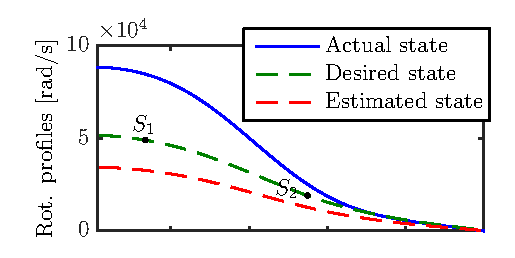
\includegraphics{imene_figs/fig13a}\adjustbox{raise=3.8em,lap=-7em}{$t = 0.50$\,s \ (a)} \\[-0.3em] % Goum18ln
	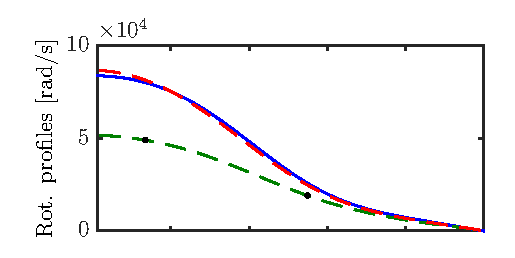
\includegraphics{imene_figs/fig13b}\adjustbox{raise=6.8em,lap=-7em}{$t = 0.51$\,s \ (b)} \\[-0.3em] % Goum18lln
	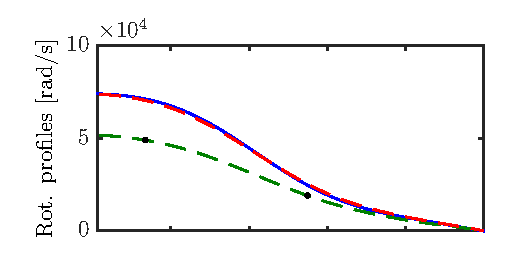
\includegraphics{imene_figs/fig13c}\adjustbox{raise=6.8em,lap=-7em}{$t = 0.52$\,s \ (c)} \\[-0.3em] % Goum18llln
	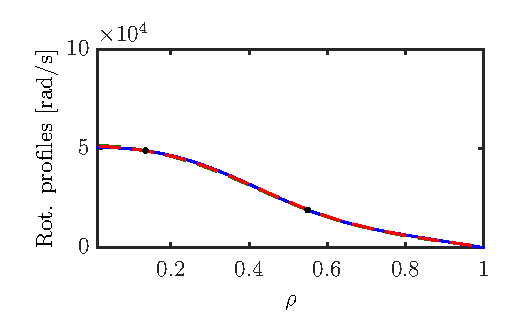
\includegraphics{imene_figs/fig13d}\adjustbox{raise=9.7em,lap=-7em}{$t = 0.57$\,s \ (d)} % Goum18lllln
	\caption{Time evolution of the rotation in the model as it evolves toward the target values and its estimate at 4 different times. The green profile is the targeted rotation profile. }
	\label{fig:rot18}
\end{figure}


Figure~\ref{fig:rot18} shows the rotation profile, comparing the actual profile, the desired profile, and the profile estimated by the observer.  Four different times are shown: $0.5$\,s (at which time the controller is turned on), $0.51$\,s, $0.52$\,s and $0.57$\,s respectively. The two sensors locations are indicated in the figure, and it can be noticed that the targeted profile is reached in less than $0.1$\,s.
\begin{figure}
\centering
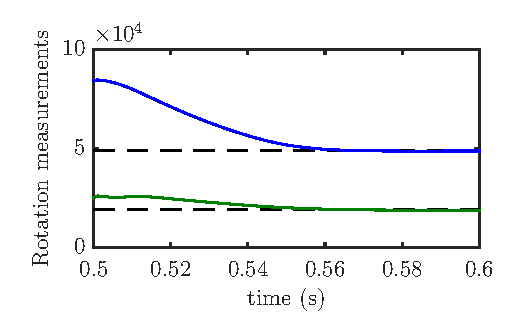
\includegraphics{imene_figs/fig14} % Goum20n 
\caption{Time evolution of the rotation measurement at the two sensor points. The dashed lines represents the desired measurements at these latter locations. }
\label{fig:rot20}
\end{figure}    

Figure~\ref{fig:rot20} shows the time evolution of the rotation measurement focused at the two sensor points located at the core and towards the edge of the plasma only. The outputs track the desired values well after about $50\,ms$. 
\begin{figure}
	\centering
	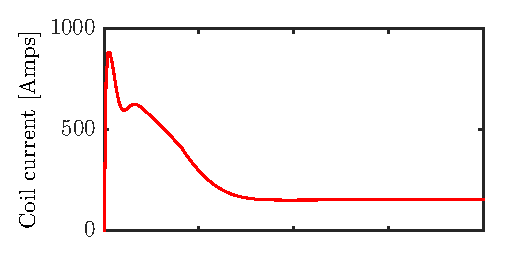
\includegraphics{imene_figs/fig15a} \adjustbox{raise=7.4em,lap=-2.8em}{(a)} % Goum19ln
	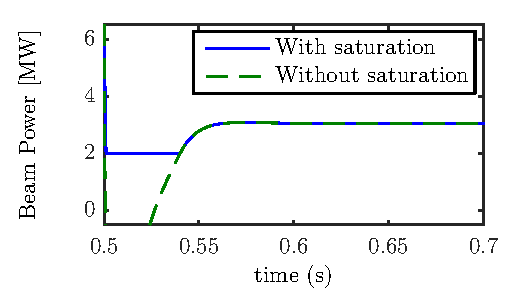
\includegraphics{imene_figs/fig15b} \adjustbox{raise=3.2em,lap=-2.8em}{(b)}
	\caption{Time evolution of the coil current and the overall beams power and its saturation, needed to reach the 1st desired profile }
	\label{fig:rot19}
\end{figure} 

Figure~\ref{fig:rot19} represents the requested inputs (coil current and overall beam power) needed to reach the desired profile of Figures~\ref{fig:rot18} and \ref{fig:rot20}. It can be noticed that the current does not saturate whereas the beam power does.

Because the initial profile (Figure~\ref{fig:rot18}(a)) before turning the controller on, is above the targeted profile  (Figure~\ref{fig:rot18}(d)), and the difference between the two profiles is higher towards the core of the plasma (where the beam power acts), the controller tries to first push the power down starting from $6$\,MW at the initial state before controlling, up to $2$\,MW when it hits saturation. The green dashed line in Figure~\ref{fig:rot19} shows how the controller would apply the beam power if no saturation was in effect. During the rapid decrease of the beams power, the controller increases the coil current in order to increase the drag and forces rapid deceleration towards the edge of the plasma.  
The controller and the actuators, when they can be activated instantaneously, enable the rotation profile to reach its target about 2 times faster (about 60\,ms) than the momentum diffusion time (about 100\,ms).

\subsection{Computational approach for TRANSP}
In order to predict the toroidal rotation for NSTX, the TRANSP code running in predictive mode is used for a given beam power and coil current. It also takes as inputs the time histories of the plasma boundary shape, plasma current, electron and ion (Chang-Hinton model \cite{Changhinton}) temperature and density profiles and the momentum diffusivity coefficient.

The actuator commands needed for closed-loop rotation control simulations are entered into the TRANSP code, which serves as a plasma simulator for testing the present controller. For more details on the TRANSP implementation, see \cite{Boyer15}.

\subsection{Simulation with PWM}
The discretized controller is now applied to the reduced-order model and the TRANSP predictive model, considering all the constraints listed in Section~\ref{constraints} for both actuators. The main difference with Section~\ref{noPWM} will be that instead of applying the exact beam power numerical value as requested by the controller, each of the 3 beams will be modulated individually while satisfying all the constraints.

At the beginning of each duty cycle, the controller sets the requested power. During the duty cycle, the beams switch on and off at most once to minimize the number of switches. Because of this and the 10\,ms refractory period, the exact requested power cannot always be met.

Durations greater and smaller than 10\,ms are chosen to compare output results for different duty cycle durations. The longer the duty cycle, the better for the device because it means less commands switches so less fatigue, but a longer duration introduces a longer controller lag which impairs performance.
  
\begin{figure}
	\centering
	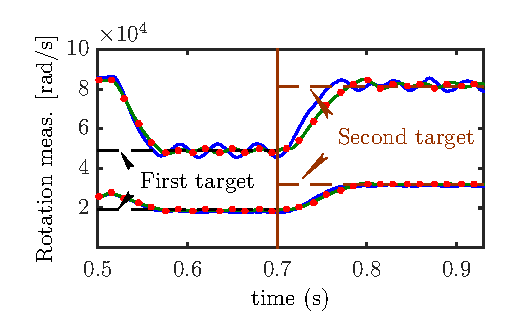
\includegraphics{imene_figs/fig16} % Goum14ln
	\caption{Comparison of the rotation measurements when PWM is applied for both the reduced-order model (green lines) and the TRANSP predictive model (blue lines). The red dots represents the cycle times (every $0.015 s$).}
	\label{fig:rot14}
\end{figure}

\begin{figure}
	\centering
	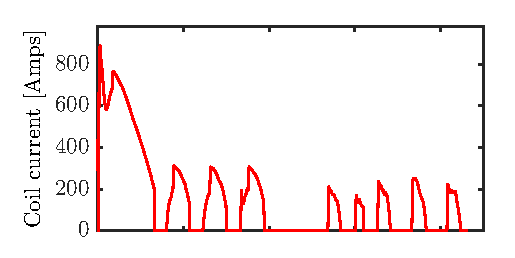
\includegraphics{imene_figs/fig17a} \adjustbox{raise=7.3em,lap=-2.8em}{(a)} \\[-0.5em] % Goum15ln
	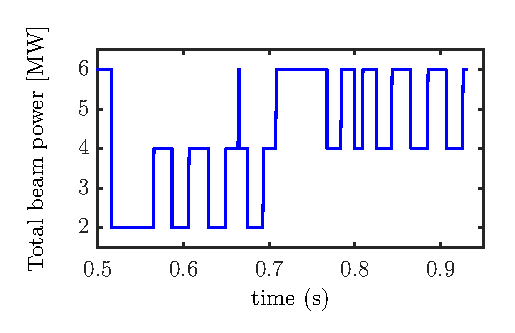
\includegraphics{imene_figs/fig17b} \adjustbox{raise=3.6em,lap=-2.8em}{(b)}
	\caption{Time evolution of the coil current and the overall beams power (cycle time $0.015  s$).}
	\label{fig:rot15}
\end{figure}

Figure~\ref{fig:rot14} compares the rotation measurements when the PWM controller is applied to both the reduced-order model and the TRANSP predictive model in order to reach two targets, one at $t = 0.5$s, and the other starting at $t=0.7$s.
Before $t=0.5$\,s, both models are not controlled (open loop), the measurements are already shown to be the steady-state values shown in Figure~\ref{Goum12}.
At $t = 0.5$\,s, the controller is turned on (closed loop), and the goal is to reach the first target profile measurement points defined by the two red dots in Figure~\ref{fig:rot11}. At $t = 0.7$\,s, the  target profile changes to the second one which is defined by the two blue dots in Figure~\ref{fig:rot11}.
The green line represents the reduced-order model outputs, the blue line represents the TRANSP model. The oscillations are due to the modulations that occurs on each of the beam power source. The total beam power is represented in Figure~\ref{fig:rot15} (right). The coil current in this case (Figure~\ref{fig:rot15} left) changes to compensate for when the beam power is too high in order to decrease the toroidal rotation and thus limit the rotation overshoot.
In this example, the duty cycle duration is 15\,ms which gives a reasonable amplitude of oscillation while reaching both targets within the momentum diffusion time ($0.1 s$).

Figure~\ref{fig:rot16} and Figure~\ref{fig:rot17} represent the same quantities as in Figure~\ref{fig:rot14} and Figure~\ref{fig:rot15} respectively, but for a different duty cycle duration (6\,ms) which is smaller that the the 10\,ms refractory period.
The resulting rotation measurements are more oscillatory but the amplitude is better damped. The trade off is that we have to activate the controller more often and thus formulate more requests to the real device.

The reduced-order model in both cases is very close to the TRANSP which again shows that the simplified model gives us a good qualitative approximation of the TRANSP rotation prediction model.

\begin{figure}
	\centering
	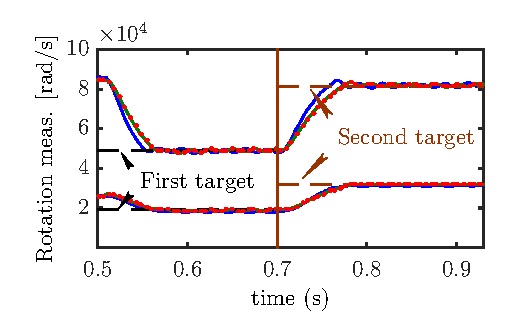
\includegraphics{imene_figs/fig18} % Goum16ln
	\caption{Comparison of the rotation measurements when PWM applied for both the reduced-order model (green lines) and the TRANSP predictive model (blue lines). The red dots represents the cycle times (every $0.006 s$).}
	\label{fig:rot16}
\end{figure}

\begin{figure}
	\centering
	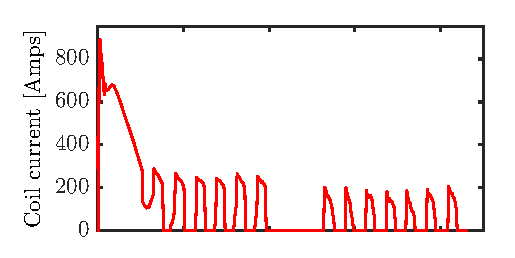
\includegraphics{imene_figs/fig19a} \adjustbox{raise=7.3em,lap=-2.8em}{(a)} \\[-0.5em] % Goum17ln
	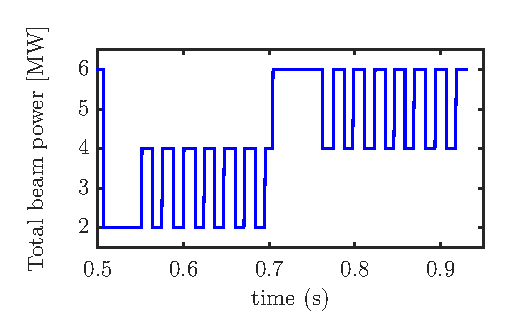
\includegraphics{imene_figs/fig19b} \adjustbox{raise=3.6em,lap=-2.8em}{(b)}
	\caption{Time evolution of the coil current and the overall beams power (cycle time $0.006 s$). }
	\label{fig:rot17}
\end{figure}


\section{Summary and conclusions}
\label{sec:conclusions}

In the above plasma control demonstrations, a simple reduced-order model has been built to capture the rotational toroidal momentum balance, applied specifically to the NSTX device. The neutral beam injection and the neoclassical toroidal viscosity are considered in this model as actuators. The output from the present model have been compared with analysis from a predictive model of NSTX and were found to be in good agreement.
Based on this simplified model, a complete feedback control design using optimal control techniques as shown above and enables controlling the plasma about a desired profile. This reduced-order controller was then tested using the NSTX predictive model and enabled the rotation profile to reach the desired profile.

Generally, broader toroidal rotation profile brings more stability to the plasma \cite{Sabbagh10} and local rotation shear can affect MHD modes  \cite{Gerhardt09}. In the new upgrade of the device, NSTX-U, three additional NBI sources (Figure~{\ref{NBI_pics}}) will provide significantly different torque profiles which can affect a broader region of the plasma, specifically towards the edge and can change the shear locally. In this case, the controller can use these added beam sources allowing significantly greater control of plasma instabilities.
Furthermore, while only the $n = 3$ applied field configuration was considered for the NTV actuator, it is possible to include different applied field spectra which can change the NTV torque profile. For example, an $n=1$ field configuration can allow a deeper penetration of this torque profile which will expand the capability of rotation control.

The present controller was designed using models tuned to match experimental data. A next step could be to develop control-oriented models directly from simulations. This capability would have a large impact: fewer experiments would be needed to calibrate the models/controllers, and more importantly, one could predict actuator requirements (e.g., amplitude, bandwidth, latency), and any inherent performance limitations for future machines such as ITER.
These control-oriented models such as those being developed using TRANSP for NSTX-Upgrade will be tested for their robustness in producing greater range of target profile shapes. 

 
\ack 

This work was supported by the U.S. Department of Energy under contract No. DE-AC02-09CH11466 (PPPL) and U.S. Department of Energy  grant number DE-FG02-99ER54524 (Columbia University). 
\section*{References}

\bibliographystyle{unsrt}
\bibliography{pap14}


\end{document}

